%!TEX root=/home/ska124/Dropbox/Thesis/thes-full.tex

%%%%%%%%%%%%%%%%%%%%%%%%%%%%%%%%%%%%%%%%%%%%%%%%%
%
%     Chapter 5
%
%%%%%%%%%%%%%%%%%%%%%%%%%%%%%%%%%%%%%%%%%%%%%%%%

\chapter{Evaluation}
\label{chap:evaluation}
This chapter evaluates the performance of the \AC\ described in Chapter~\ref{chap:ac_architecture}. The evaluation is performed using the infrastructure described in Chapter~\ref{sec:simulation_infrastructure}. This chapter is divided into sections based on performance evaluations of:
\begin{itemize}[noitemsep]
	\item Comparison against a fixed granularity cache
	\item The spatial pattern predictor
	\item Adaptivity of the \AC\
	\item \AC\ versus other approaches
\end{itemize}

\section{Improved Memory Hierarchy Efficiency}
\label{sec:efficiency}
\vspace{5pt}
\noindent \textbf{Result 1:}{\emph~{\AC\ increases cache capacity by harvesting
  space from unused words and can achieve an 18\% reduction in both L1 and
  L2 miss rate.}
\\ \\
\noindent \textbf{Result 2:}{\emph~{\AC\ adaptively sizes the cache block
  granularity and reduces L1$\leftrightarrow$L2 bandwidth by 46\% and
  L2$\leftrightarrow$Memory bandwidth by 38\%.}
}
\\ \\
In this section, the bandwidth and miss rate properties of an \AC\ are compared against a conventional cache. A \textit{Fixed} cache represents a conventional cache which allocates a fixed granularity cache block on a refill request. The accuracy of the spatial pattern predictor is an important factor which governs the accuracy of the \AC\ and is evaluated separately. For the results presented in this section, cache line utilisation statistics, gathered from a prior run of the application on a conventional cache, are used to drive the predictor. This isolates the benefits of the \AC\ from the potentially changing accuracy of the spatial pattern predictor across different cache geometries. This also ensures that the spatial granularity predictions can be replayed across multiple simulation runs. To ensure equivalent data storage space, the \AC\ size is set to the sum of the tag array and the data array in a conventional cache. At the L1 level (64K), the net capacity of the \AC\ is 64K + 8*4*256 bytes and at the L2 level (1M) configuration, it is 1M + 8*8*2048 bytes. The L1 cache has 256 sets and the L2 cache has 2048 sets. 
\\ \\
\indent Fig~\ref{fig:eval_scatter_bw_64k_1m} plots the miss rate and the traffic characteristics of the \AC{}.  Since \AC{} can hold blocks varying from 8B to 64B, each set can hold more blocks by utilizing the space from untouched words. \AC\ reduces the 64K L1 miss rate by 23\%(stdev:24) for the Low group, and by 21\%(stdev:16) for the moderate group; even applications with high spatial locality experience a 7\%(stdev:8) improvement in miss rate. There is a 46\%(stdev:20) reduction on average in L1$\leftrightarrow$L2 bandwidth. At the 1M L2 level, \AC\ improves the moderate group's miss rate by 8\%(stdev:10) and bandwidth by 23\%(stdev:12).  Applications with moderate utilization make better use of the space harvested from unused words by \AC{}. Many low utilization applications tend to be streaming and providing extra cache space does not help lower miss rate. However, by not fetching unused words, the \AC\ achieves a significant reduction (38\%(stdev:24) on average) in off-chip L2$\leftrightarrow$Memory bandwidth; even High utilization applications see a 17\%(stdev:15) reduction in bandwidth.  Utilization and miss rate are not, however, always directly correlated (more details in \S~\ref{sec:adaptivity}).

\begin{figure}[ht]

  \subfloat[64K - Low]{
    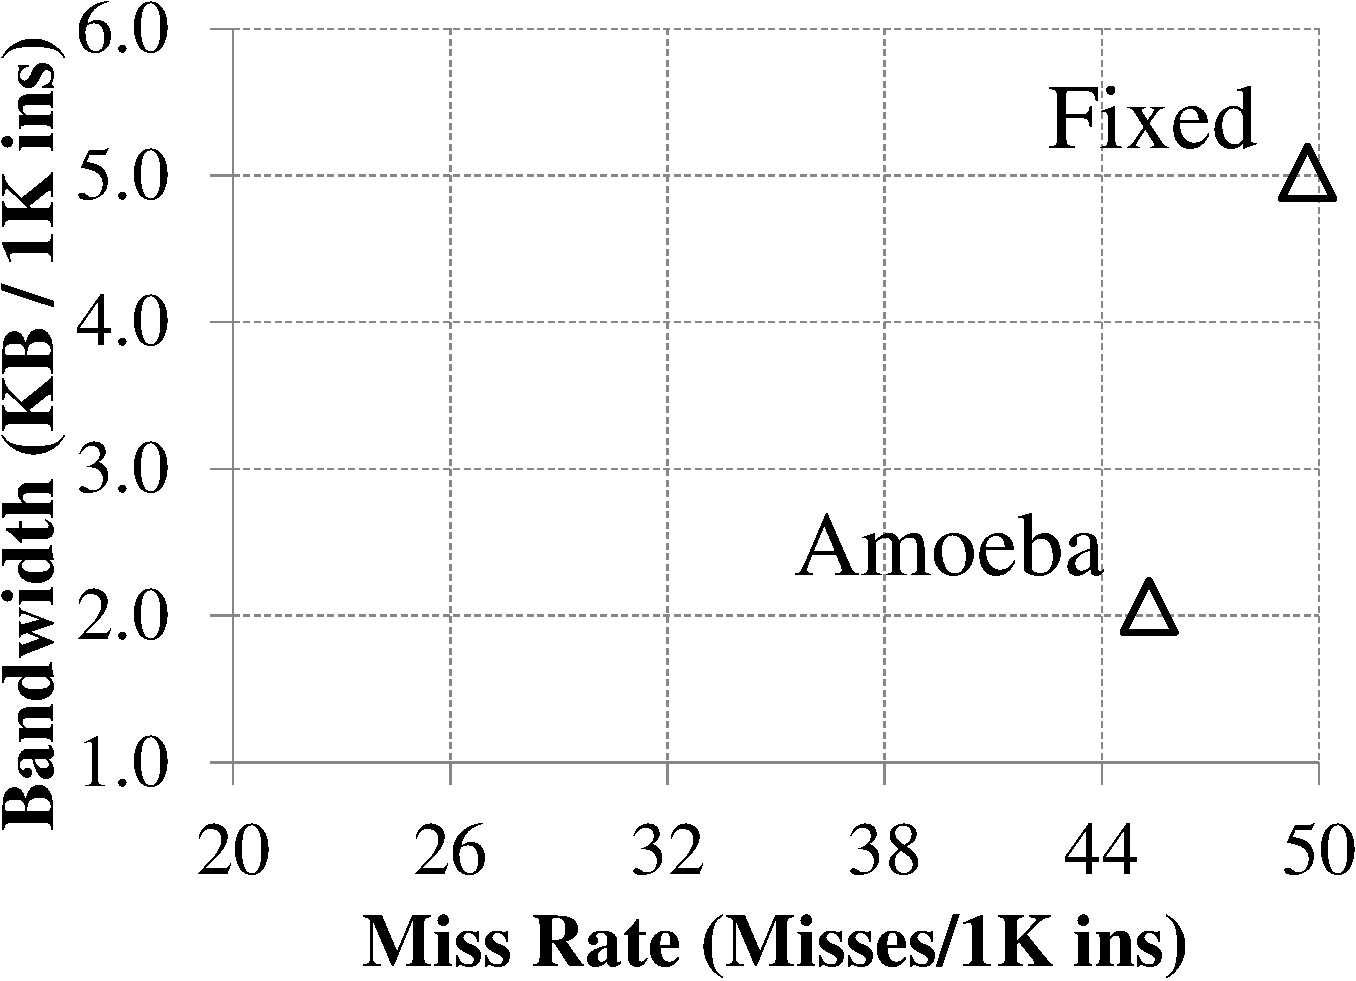
\includegraphics[width=0.48\textwidth]{files/Plots/08-Scatter_Bw_Miss_64K_low.pdf}
  }
  \subfloat[1M - Low]{
     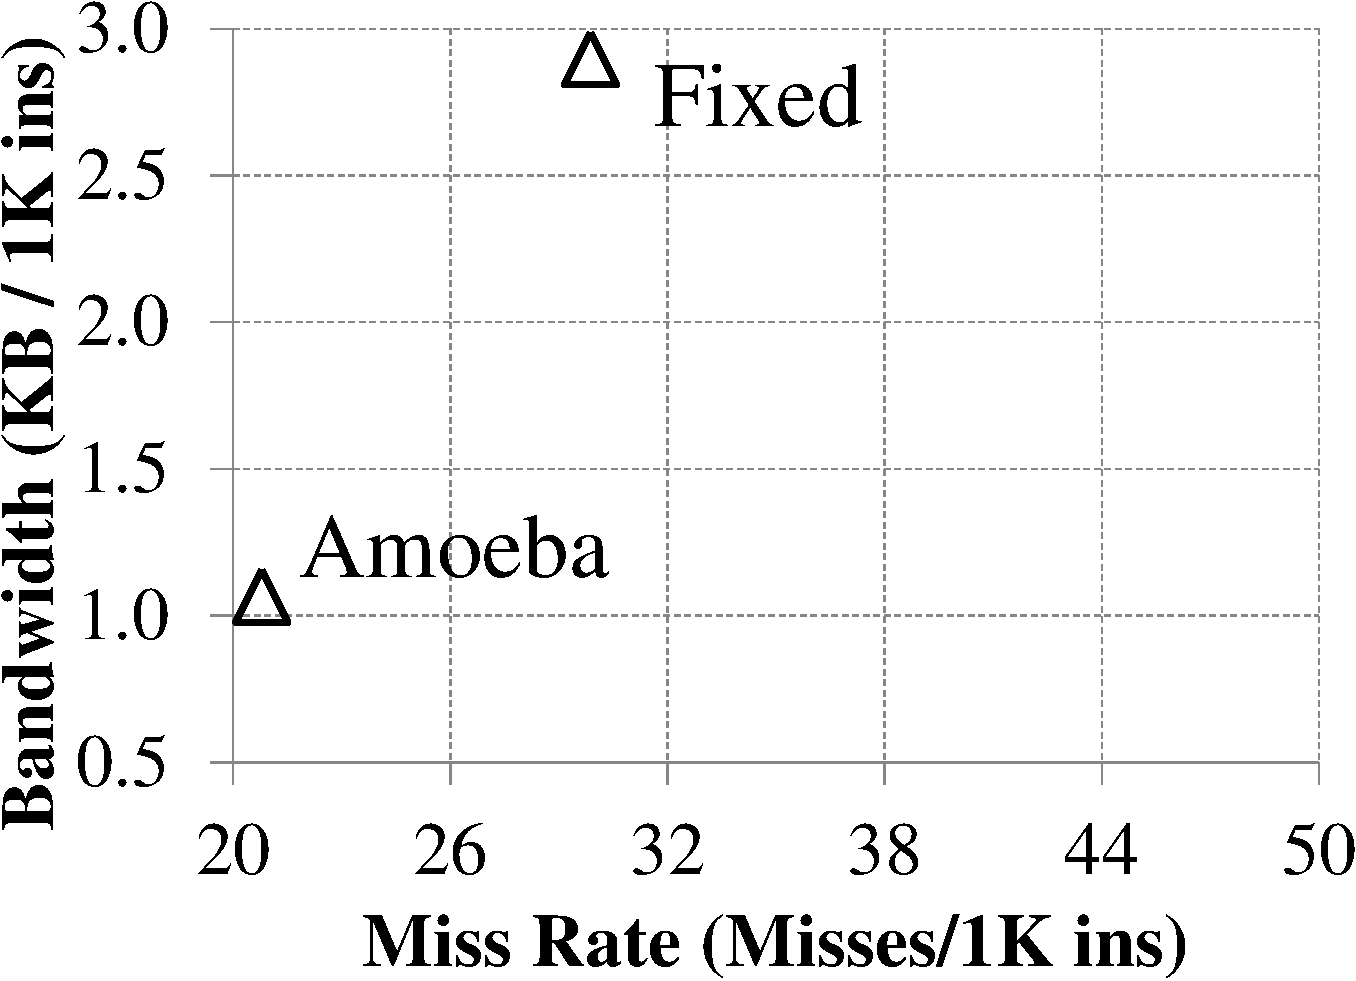
\includegraphics[width=0.48\textwidth]{files/Plots/08-Scatter_Bw_Miss_1M_low.pdf}
  }
  
  \subfloat[64K - Moderate]{
    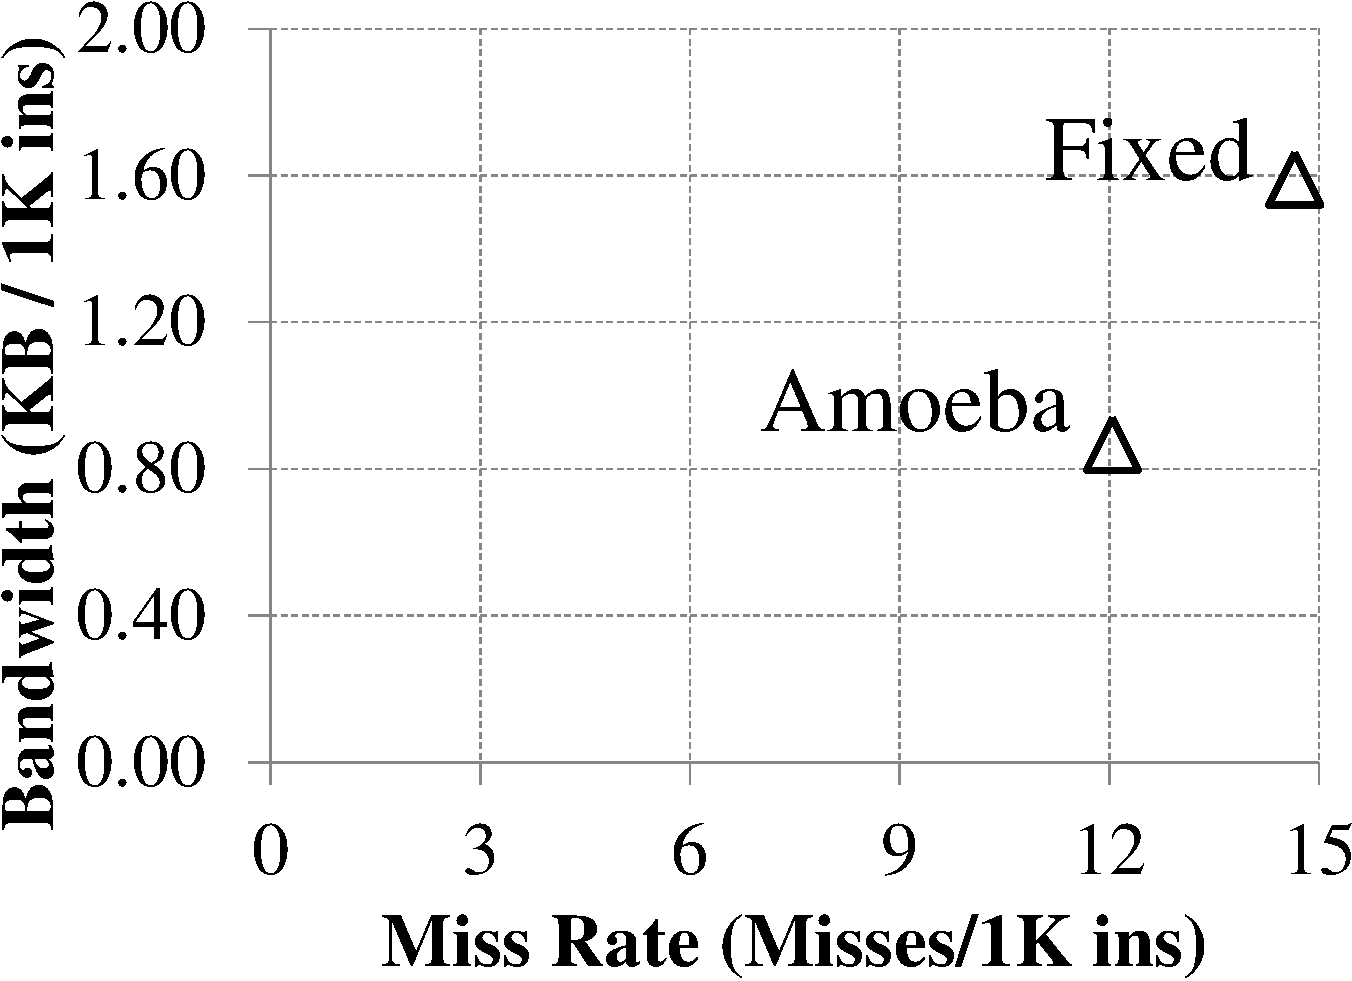
\includegraphics[width=0.48\textwidth]{files/Plots/08-Scatter_Bw_Miss_64K_mod.pdf}
  }
  \subfloat[1M - Moderate]{
     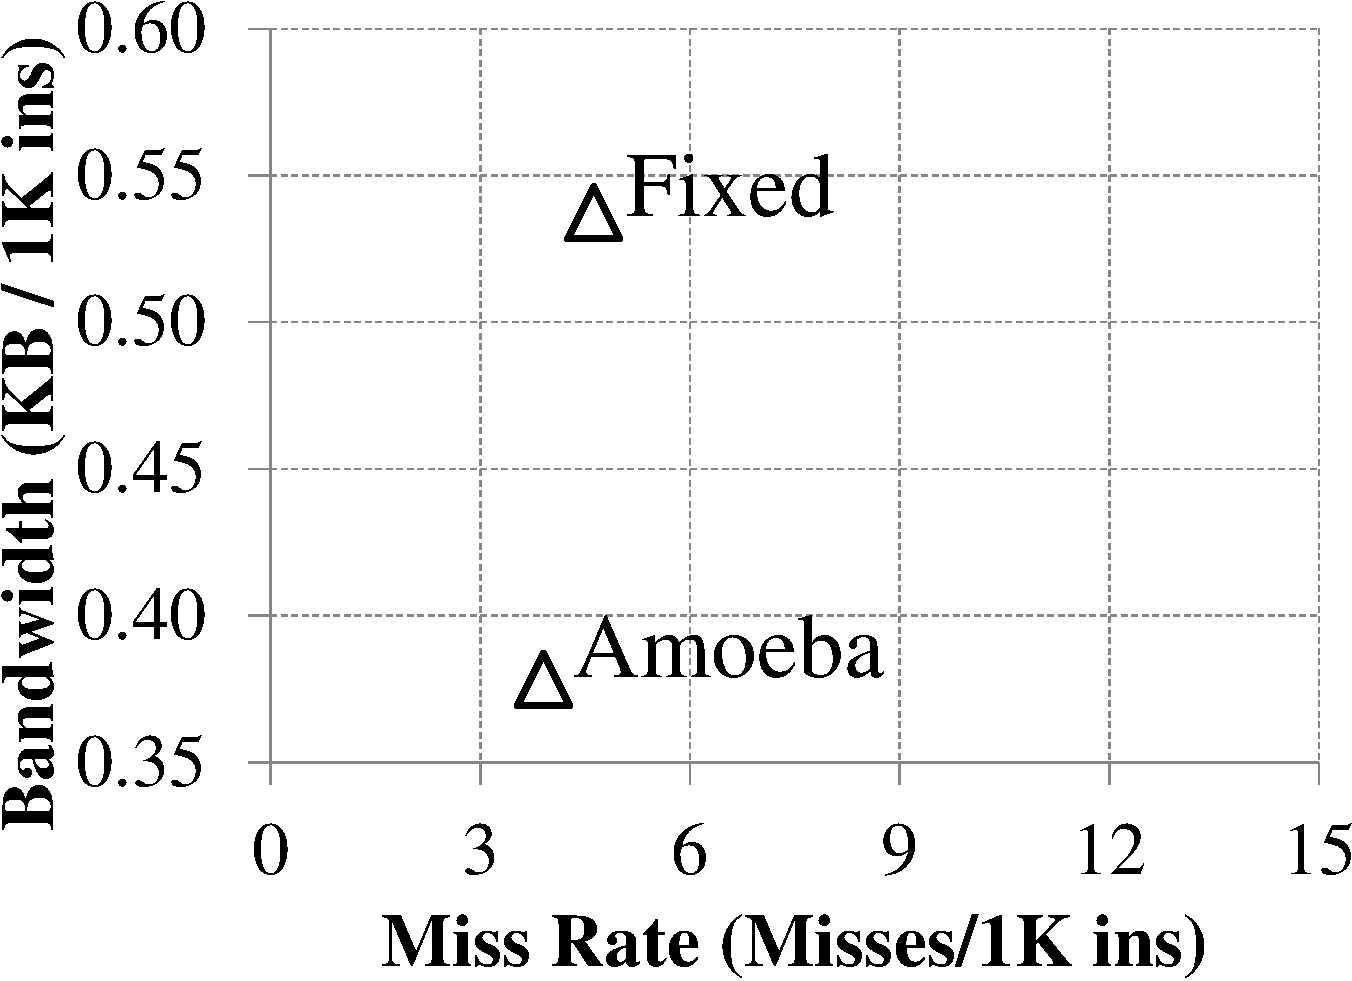
\includegraphics[width=0.48\textwidth]{files/Plots/08-Scatter_Bw_Miss_1M_mod.pdf}
  }
    
  \subfloat[64K - High]{
    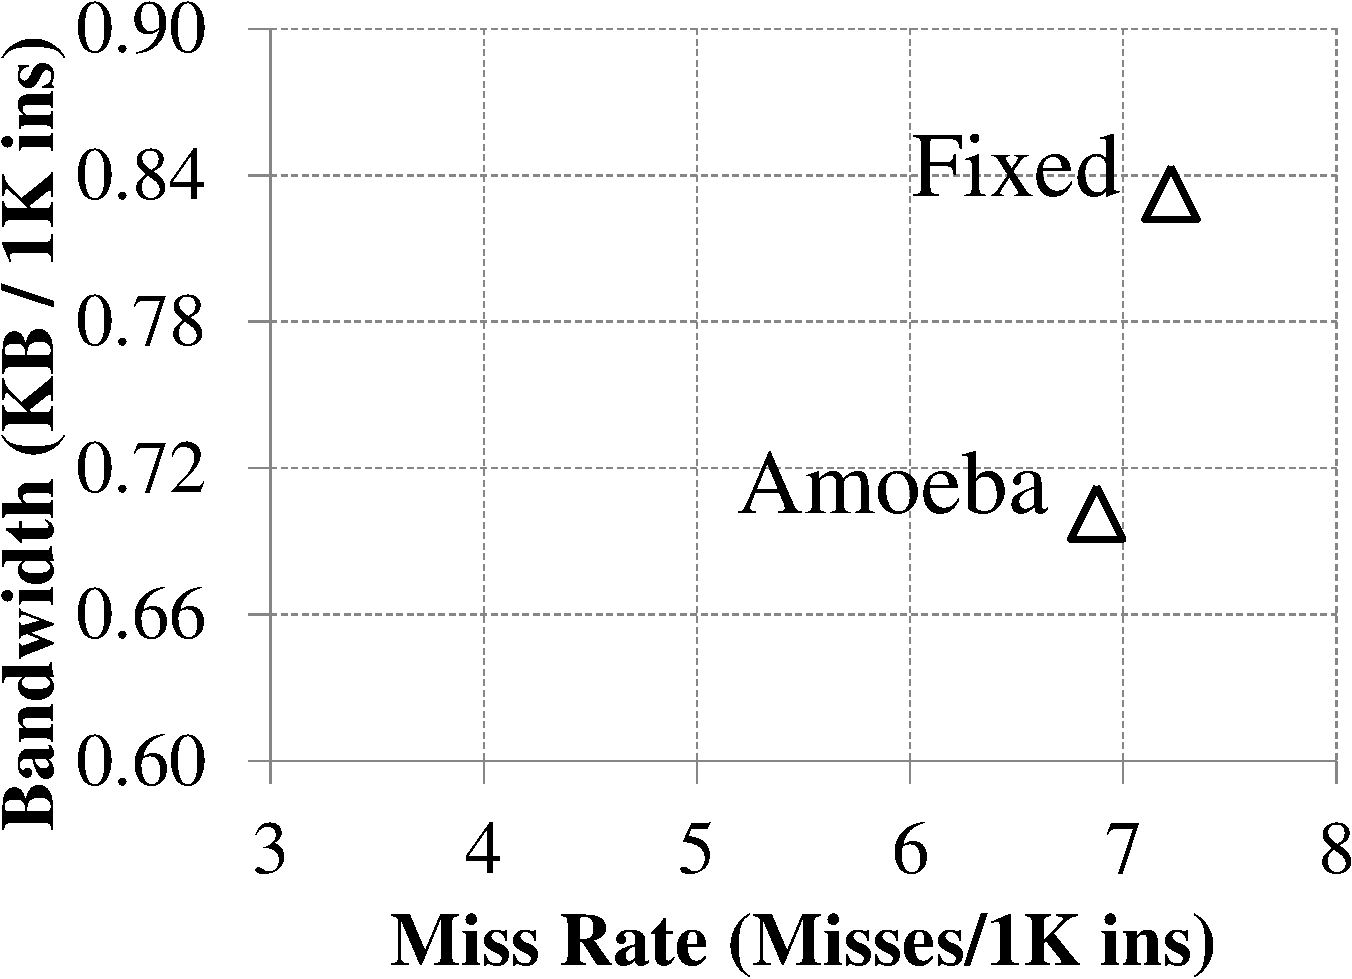
\includegraphics[width=0.48\textwidth]{files/Plots/08-Scatter_Bw_Miss_64K_high.pdf}
  }
  \subfloat[1M - High]{
     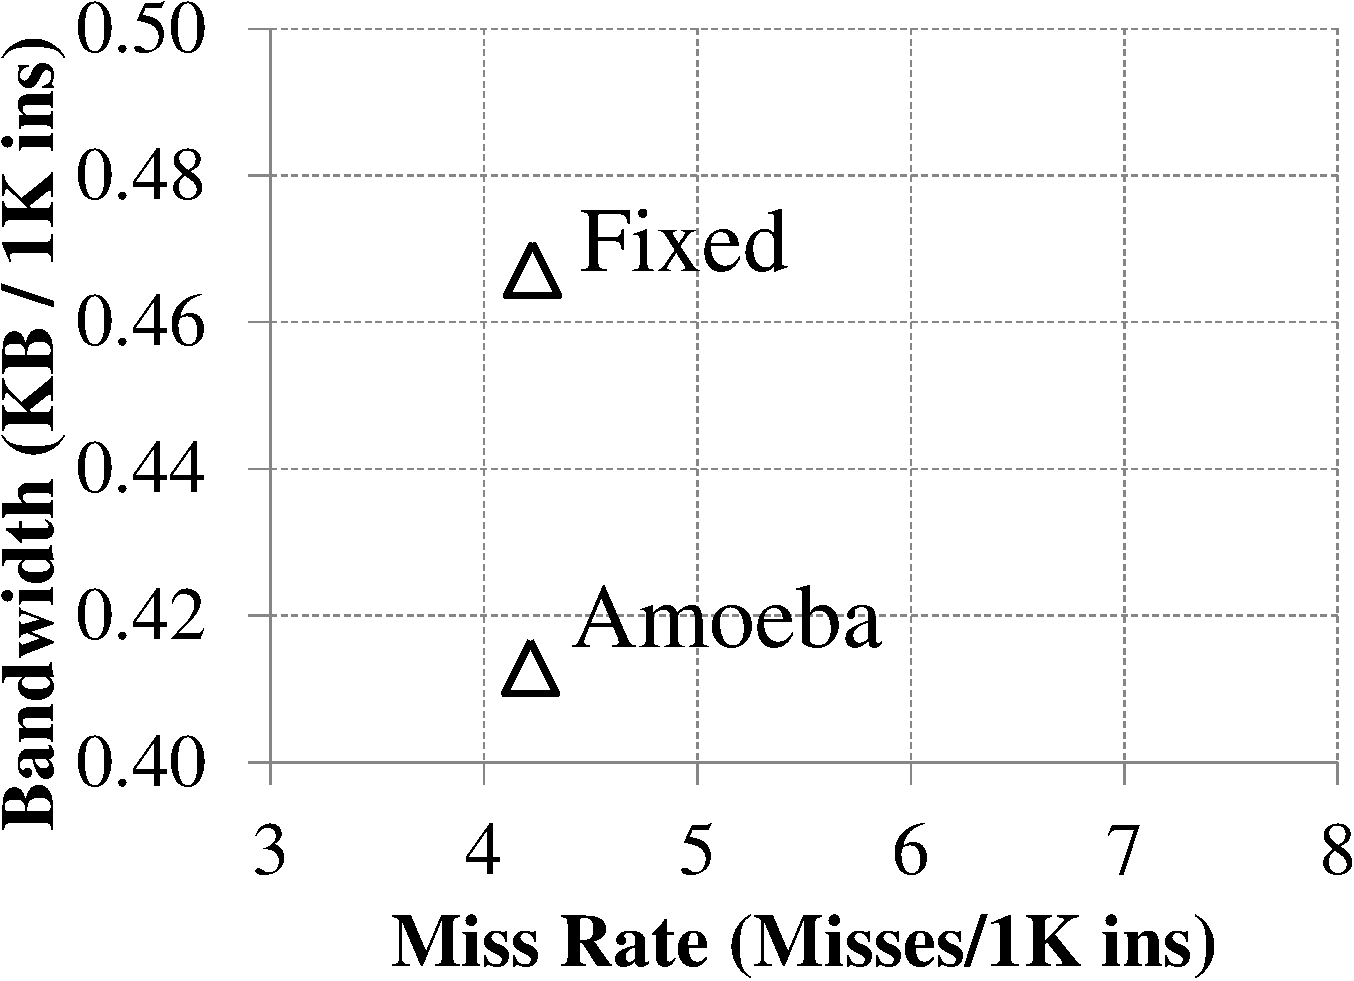
\includegraphics[width=0.48\textwidth]{files/Plots/08-Scatter_Bw_Miss_1M_high.pdf}
  }

  \caption[Bandwidth vs. Miss Rate]{Bandwidth vs. Miss Rate for a fixed granularity cache and \AC{}. (a),(c),(e): 64K, 4-wayL1 equivalent (b),(d),(f): 1M, 8-way LLC equivalent.  Markers on the plot indicate cache block size. Note the different scales for different groups.}
  \label{fig:eval_scatter_bw_64k_1m}
\end{figure}

\clearpage